\chapter{The Problem and its Background}\label{chap_problem_background}

\section{Birdsong}

Just like humans, birds made vocalization to communicate each other using the \textbf{syrinx} to produce sound instead of mammals vocal folds. These vocalizations are called birdsongs and are used at most by bird males for attraction mate or territorial defense, females also generate birdsongs but shorter and simpler than males birdsongs. Depending of the bird specie the birdsong is learned from a tutor or just inherit to them, they born with the ability to sing, but always is a signature of the bird, a way to define and characterize the individual bird. 



\subsection{Bird Calls and Syllables}

Not all vocalizations are the same. Some of them are shorter and sharper and less rhythmic, they are called \textbf{bird calls} and are used to communicate with other birds of the same or different species, to be in contact with their families and protect them. \\

On the other hand, birdsongs are usually generated by male and are more musical and longer than bird calls. In order to study them, there are three important features to be consider: sound quality, pitch trend, and number of sections.\\

To describe the sound quality of a birdsong the terms used are:

\begin{itemize}
    \item \textbf{Clear:} Where the pitch is well defined, this is something you could sing.
    \item \textbf{Buzzy:} Something like a bee, the pitch looks distorted as if it have noise.
    \item \textbf{Thrilled:} Many syllables in a sound that are too fast to count (11 elemental sounds per second).
\end{itemize}

Some birds sing with more than one quality. As an example some sings with a part buzzy and another one clear, this type is called \textbf{Partly Buzzy} .

\begin{figure}[H]
    \centering
    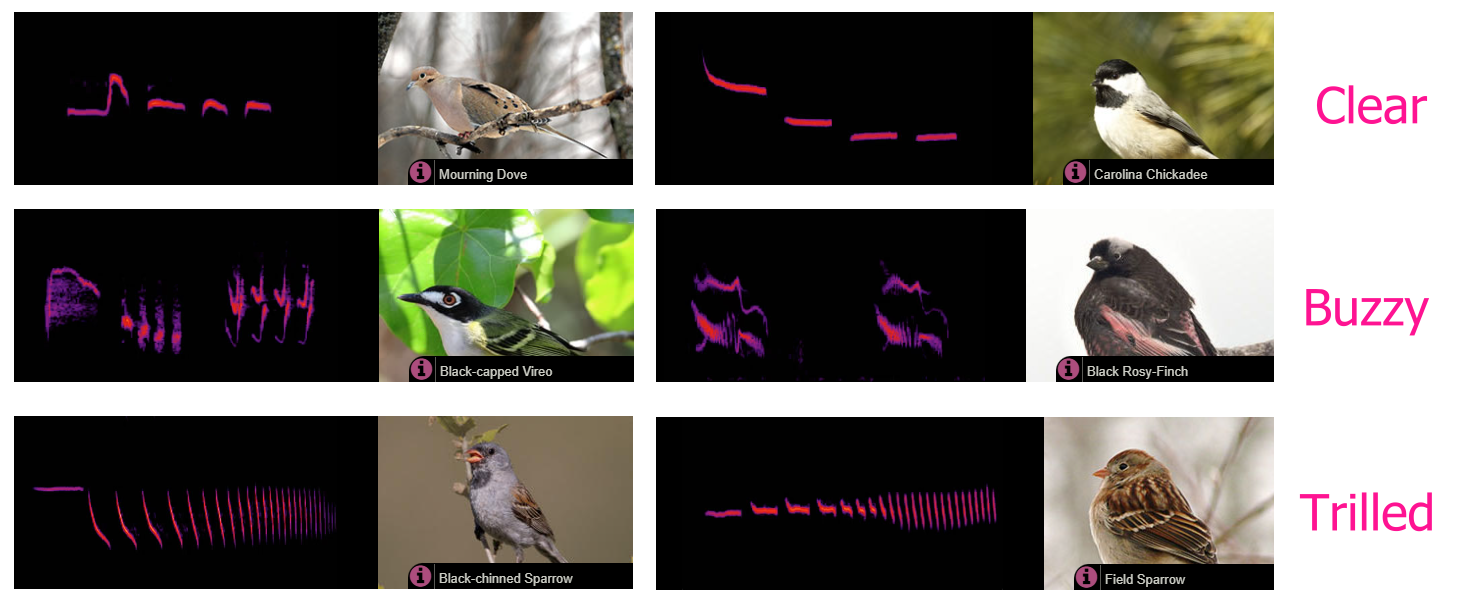
\includegraphics[scale=1.2]{Images/quality.png}
    \caption{Classification by song quality. }
    \label{fig:quality}
\end{figure}

What we call the signature of the bird is the pitch of the spectrum, even if each bird has a different spectrum they are usually classify by its overall behavior: is it steady, rising, falling, or varying, moving up and down? 

\begin{figure}[H]
    \centering
    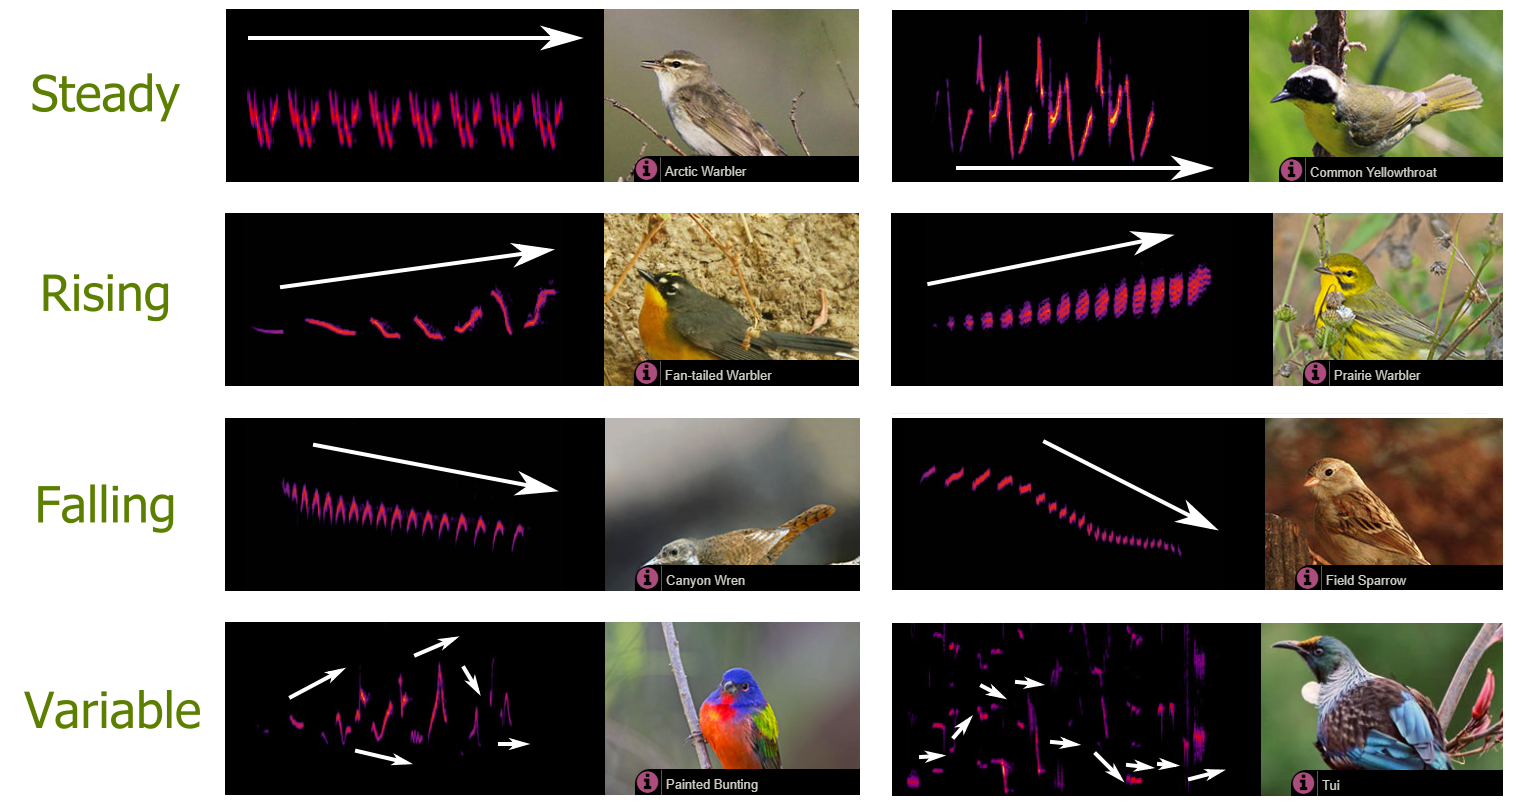
\includegraphics[scale=1.2]{Images/pitch_trend.png}
    \caption{Classification by pitch trends.}
    \label{fig:quality}
\end{figure}

In addition, the birdsongs can be break down into parts called sections, intervals where the pitch behaves in the same way, they are defined by the drastically changes in the pitch and are very utile to identify the bird. These section can be also break down into \textbf{syllables} (or elements) and \textbf{phrases}, group of consecutive syllables. 


\begin{figure}[H]
    \centering
    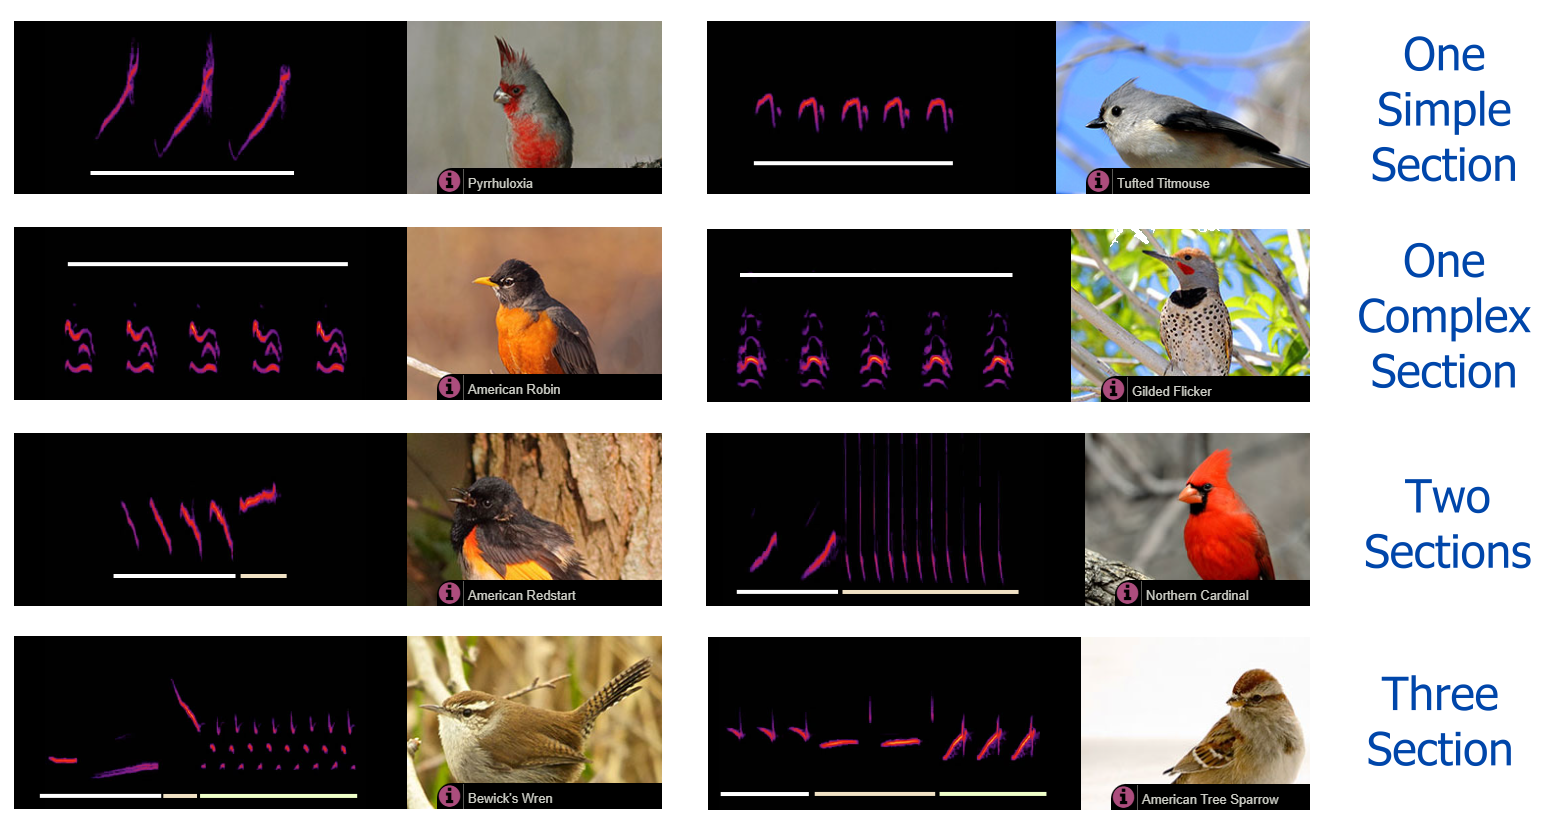
\includegraphics[scale=1.2]{Images/song_sections.png}
    \caption{Classification by number of section. This classification can be done even when the song spectrum is complex, where the signature is not quite simple and may be a composition of two pitches since many birds have two independent syrinx organs.}
    \label{fig:quality}
\end{figure}

All birds spectrograms was taking and adapted from the song learning game Bird Song Hero \cite{hero}. To deeper syllables study check the blog \href{http://earbirding.com/blog/archives/category/spectrograms}{EARBIRDING}, there you will find information about syllables classification with audio and spectrum examples and also a demonstration of how some birds of the same specie has similar spectrums.

\section{Sound Production of a Birdsong}

To understand how birds sing first let us study their anatomy, in particular the respiratory system.\\


Despite the fact that the respiratory system has many actors, to produce sound not all of them contribute. The organs involved to generate sound are the air sacs, bronchi, trachea, beak, and the \textbf{syrinx}, the main character in the sound production process.

\begin{figure}[H]
    \centering
    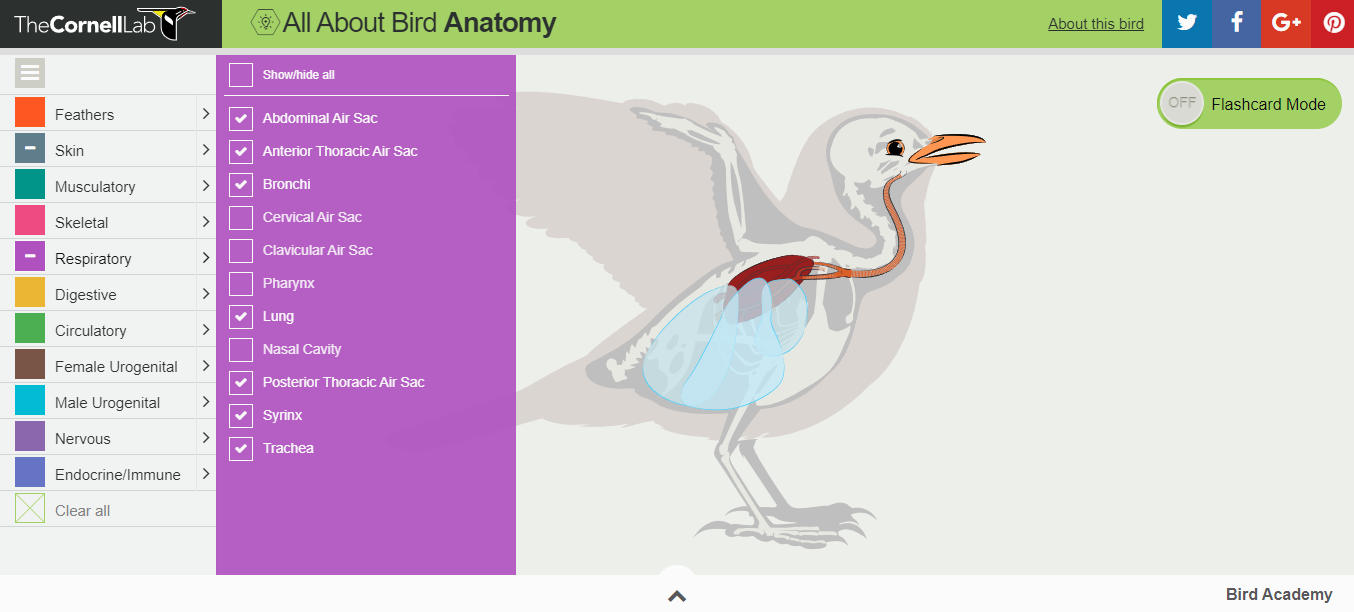
\includegraphics[width=0.85\linewidth]{Images/bird_sound_organs.png}
    \caption{Bird respiratory system anatomy. \cite{birdanatomy} }
    \label{fig:bird_sound_organs}
\end{figure}


\subsection{Syrinx}

\begin{minipage}{0.4\textwidth}
\begin{figure}[H]
    \centering
    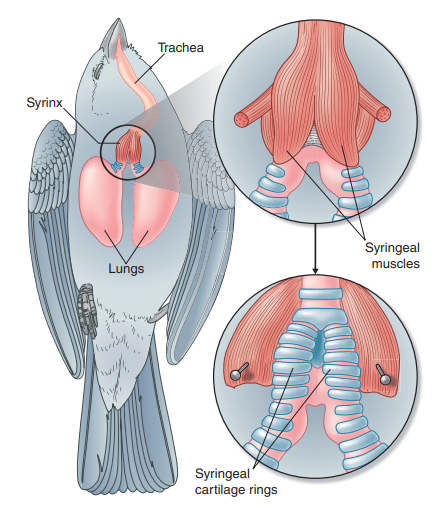
\includegraphics[scale=0.65]{Images/birdsong_paloma.png}
    \caption{Sound production actors: \textbf{the  syrinx}, air sacs, trachea, and beak. Image taken from \cite{birds_handbook}.}
    \label{fig:syrinx_paloma}
\end{figure}
\end{minipage} \hspace{50pt}
\begin{minipage}{0.48\textwidth}
The syrinx is primary sound-producing organ that birds use to generate birdsongs; it is equivalent to the mammals voice box, larynx,
and unlike humans is located where the trachea forks into the lungs, the junction where the trachea (windpipe) splits to form the two tubular bronchi as that lead to the lungs as is showed in the Figure \ref{fig:syrinx_paloma}. \\

This organ consist of two independent smalls parts of tissue, known as \textbf{labia} or membrana tympaniformis, located in major of cases at the end of the bronchus. Each labia has six pairs of muscles, called syringial muscles Figure \ref{fig:Syrinx_muscles}, that are controlled independently by a nervous system which allows to them make extraordinary and complex birdsongs, in fact they are great vocal gymnast.
\end{minipage}

%\vspace{5pt}

\begin{figure}[H]
    \centering
    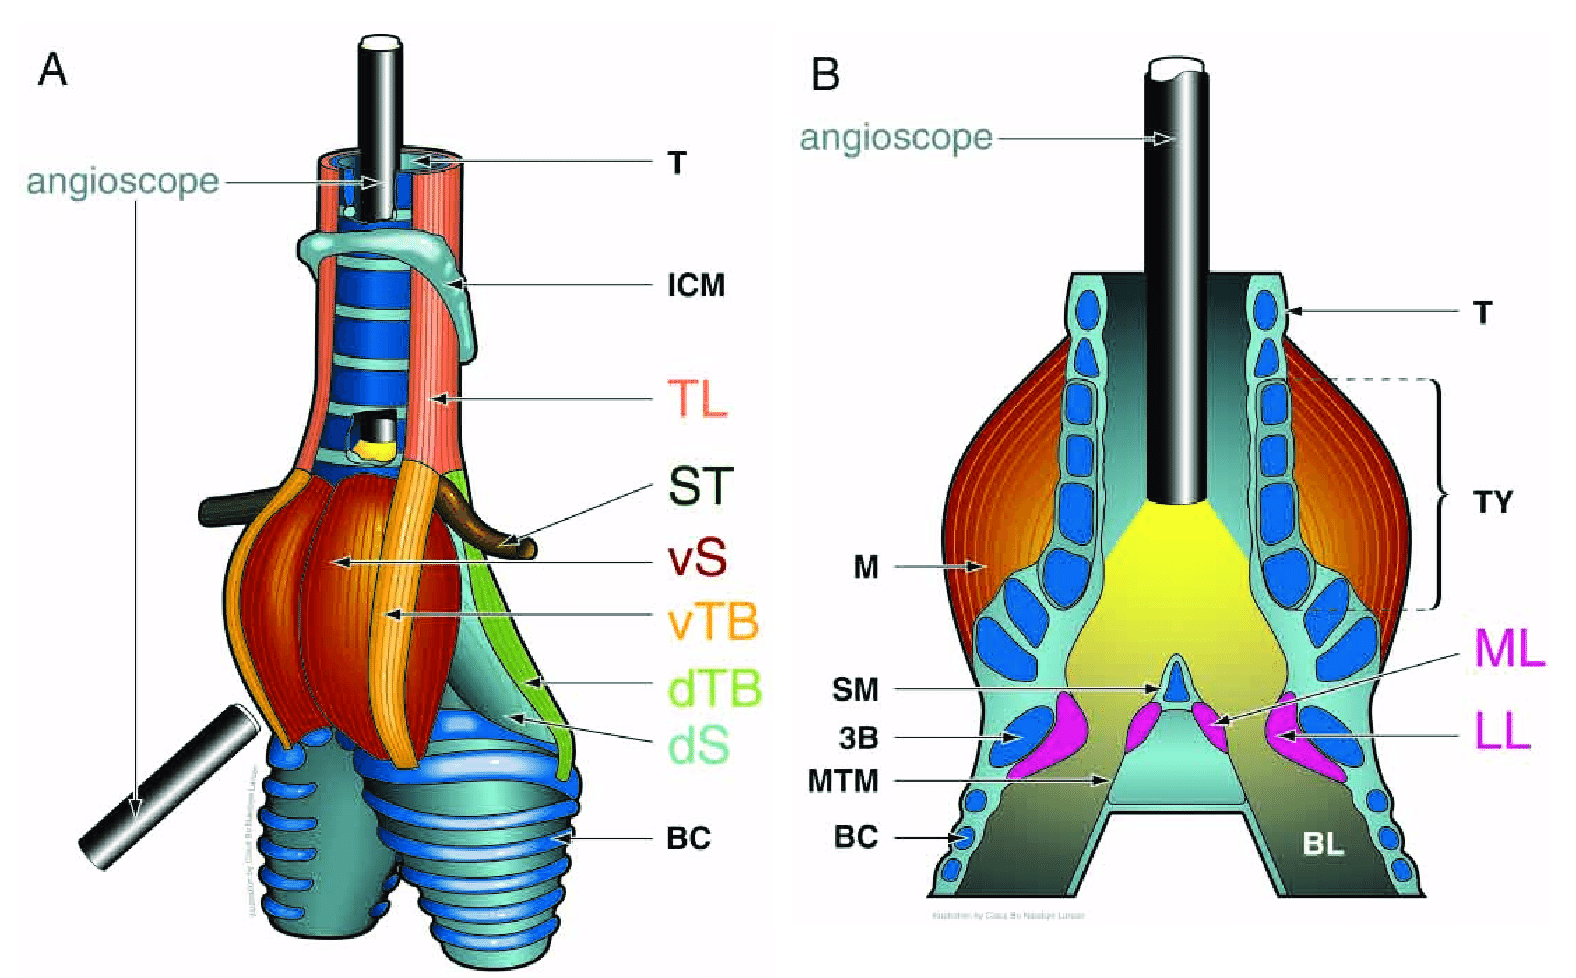
\includegraphics[scale=0.3]{Images/syrinx_muscles.png}
    \caption{Syringeal muscles \cite{Syrinx_muscles}.}
    \label{fig:Syrinx_muscles}
\end{figure}

Since each labia is independently controlled, each one can produces different sounds making the bird singing different syllables at the same time, as shown in the Figures \ref{fig:syrinx_bird} and \ref{fig:syrinx_gif}. 

\begin{figure}[H]
    \centering
    \animategraphics[loop,width=0.85\linewidth]{32}{Images/spectrum/birdsong_spectrum-}{0}{32}
    \caption{Independent syrinx oscillations and its corresponding spectrograms  \cite{birdsongs_cornell}}
    \label{fig:syrinx_gif}
\end{figure}


To produce the sound, the labia oscillations modulates the air passing through them, which comes from the air sac, and then goes to the trachea and expel by the beak, they attenuate the sound amplitude of a particular frequency and enhance the pitch.







\begin{figure}[H]
    \centering
    \animategraphics[loop,width=0.8\linewidth]{13}{Images/syrinx/birdsong_syrinx-}{0}{13}
    \caption{Syrinx oscillations. Many birds have two independent syrinx to modulates the air and produces birdsongs, some of them are able to control each syrinx an generate complex sounds as is showed in this figure.}
    \label{fig:syrinx_bird}
\end{figure}







\subsection{Physics of a Birdsong}

As was discussed in the section \ref{subsec_sound_waves}, a sound wave is the propagation of a pressure perturbation in an elastic medium such as air. This perturbation is produced by the vibration of molecules that generates local changes of density such that lead to changes in pressure, as is shown in the following Figure \ref{fig:air_motion}. The density perturbation is proportional to the air displacement velocity and the initial density.\\

The pressure perturbation is generated by a vibrating sound source that moves forward and back to spread out the first medium particles, then they push their surrounding particles and the perturbation is propagated. The medium is a series of particles interconnected and interacting that must be able to transmit energy (an elastic medium).

\begin{figure}[H]
    \centering
    \animategraphics[loop,width=\linewidth]{17}{Images/birdsong/birdsong-}{0}{17}
    \caption{\cite{birdsongs_cornell}}
    \label{fig:air_motion}
\end{figure}



The usual sound wave representation is the \textbf{waveform} where the amplitude of the wave is plotted as a function of time, the amplitude represents the sound loudness. Another important sound feature is the frequency, that have information about the pitch, that is define as the rate at which sound waves are produced, sounds with higher frequencies than 20.000 Hz are called ultrasonic while frequencies below are known as infrasonic. The frequency inverse is the period $T=1/f$, the amount of time it takes to complete one wave cycle\footnote{when two successive crests (or through) past an specific point} 

\begin{figure}[H]
    \centering
    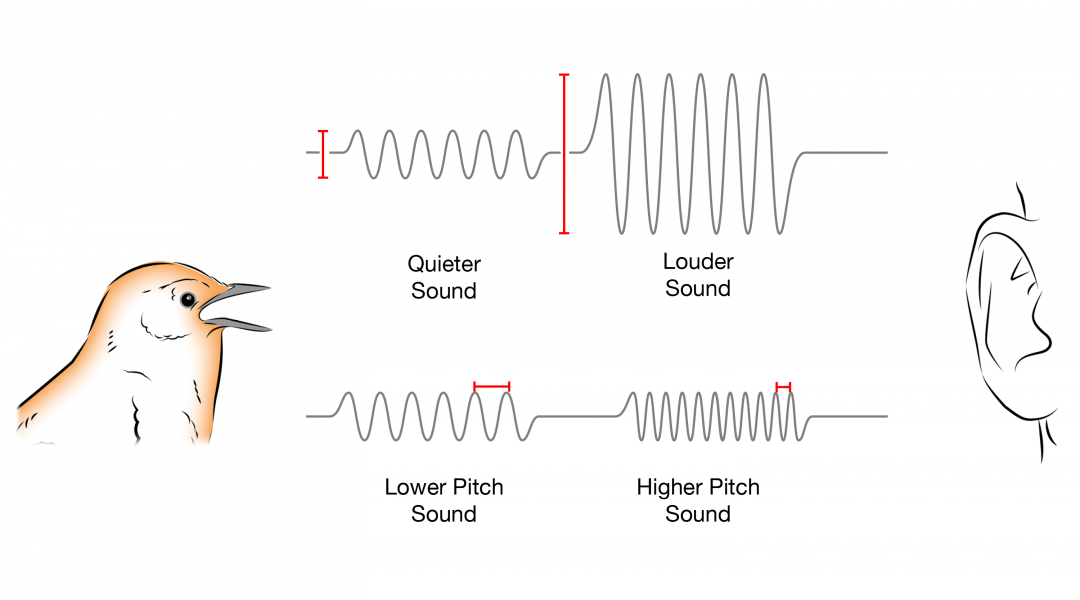
\includegraphics[scale=0.35]{Images/sound_pitch.png}
    \caption{Sound pitch \cite{birdsongs_cornell} }
    \label{fig:sound_pitch}
\end{figure}

In physiology, sound is defined as how humans receive the  sound waves and how is their perception by the brain. The human eardrums are night and day hit by sounds, as response they vibrate and convert these vibrations into electrical signals that travel to the brain and are interpreted as sound. The brain perception allows to us to distinguish and classify the signal by their pitch or loudness.

\begin{figure}[H]
    \centering
    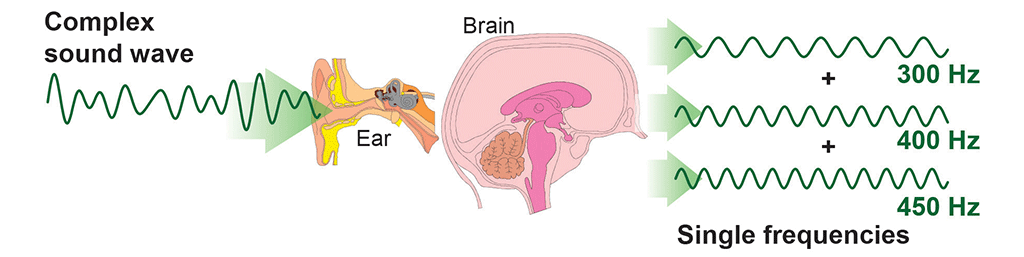
\includegraphics[width=0.9\linewidth]{Images/complex_sound.png}
    \caption{Sound human brain understanding \cite{sound_pasco} }
    \label{fig:}
\end{figure}


%https://academy.allaboutbirds.org/features/birdanatomy/

% \textbf{What is it?}
% \textbf{How does it work?}
% \textbf{Importance}


\section{Motor Gestures}


\begin{figure}[H]
    \centering
    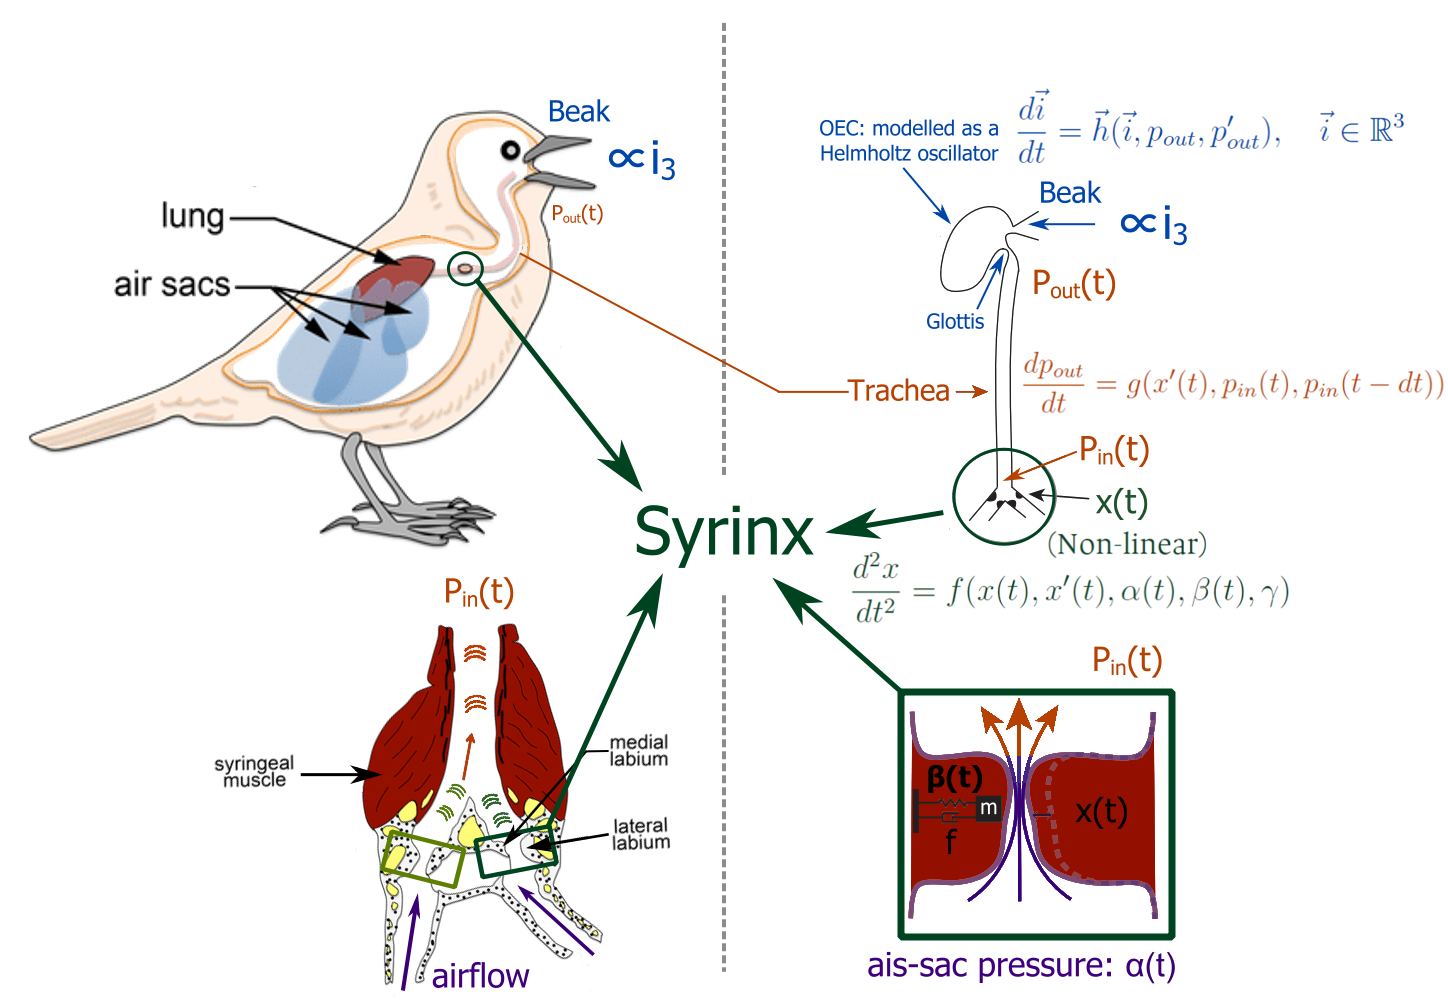
\includegraphics[width=0.85\linewidth]{Images/model.png}
    \caption{Schematized view of a dynamical systems model describing syringeal labial dynamics and tracheal vocal-tract filtering. The syringeal membrane was modeled as a mass ($m$) with external pressure ($\alpha$) and a restitution (spring) constant ($\beta$). Here: $\gamma$, time constant; $r$ , reflection coefficient of the trachea; $T=L/C$, propagation time along trachea; $v$, proportional to the mean velocity of the flow; $y=x'$, velocity. Images taken and adapted from \cite{complete_model} and \cite{siryx_image}.}
    \label{fig:bird_sound_organs}
\end{figure}

The most complete and tested physical model to simulate the birds sound production is the \textbf{motor gestures model}. It has been developing in the Dynamical System Lab, lead by professor G. Mindlin of the National University of Buenos Aires (UBA). The model simulate the bird sound production system by modeling the syrinx, trachea, Oro-Oesophageal Cavity (OEC), glottis, and beak with ordinary differential equations (ODEs). 


\subsection{Timeline}

The described bird's vocalization model was developed based on the the human vocals folds literature models. The first model of human vocal folds date at 1988 and was created by Titze, \cite{Titze1998}, where he studied how the muscles movement generate a pressure wave that yields to a vocalization due to the muscles oscillations. 

\begin{minipage}{0.55\linewidth}
This model consider the vocal folds as a simple mass-spring oscillator, a second order differential equation, with a nonlinear driven force 
\begin{equation*}
    m \xi'' + b \xi' +  k\xi = f(\xi(t), \xi'(t), t)
\end{equation*}    
where $\xi, \xi',$ and $\xi''$ are the wall vocal fold position, velocity and acceleration, respectively, $m$ the mass, $k$ the stiffness, $b$ the damping, $f$ the driving force, and $t$ the time. The study of the dynamical behavior of the Titze model shows that the oscillation occurrence depends of the driving force $f$ and the velocity term, which involves the damping constant and vocal folds walls velocity. Since this model is basic it has great interpretability and has been used as a toy model to simulate human and animal vocalizations. 

\end{minipage}\hspace{10pt}
\begin{minipage}{0.4\linewidth}
\begin{figure}[H]
    \centering
    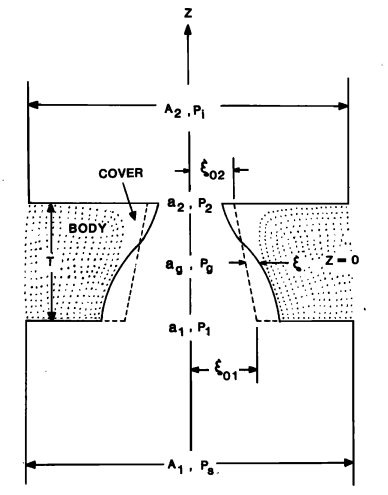
\includegraphics[width=0.9\linewidth]{Images/tatzi.png}
    \caption{Frontal section of body-cover model, vocal folds, used for small-oscillation analysis \cite{Titze1998}, a toy model.}
    \label{fig:titze}
\end{figure}
\end{minipage}

\vspace{10pt}


\begin{minipage}{0.55\linewidth}
\begin{figure}[H]
    \centering
    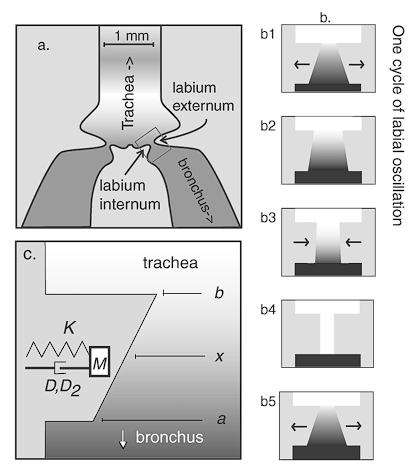
\includegraphics[width=0.9\linewidth]{Images/simple_gestures.png}
    \caption{Syrinx behavior illustration and labial dynamics. The panel (a) illustrates the present organ actors and their shape, (b) shows a representation of labial position in an oscillation cycle, and (c) is a diagram with the model terms. \cite{simple_motor_gestures_2001}}
    \label{fig:simple_gestures}
\end{figure}    
\end{minipage}\hfill
\begin{minipage}{0.4\linewidth}
Using the Titze model and studying its dynamical behavior, professor Mindlin proposed the first model to simulate birds sound production, \textbf{motor gestures for birdsongs}, making possible to create simple synthetic birds vocalizations (birdsongs). This model of bird's sound production was published at 2001 \cite{simple_motor_gestures_2001} taking advantage of the bifurcation theory ideas and applied them to the Titze model. Although Titze model was developed for human vocal folds, experimental evidence \cite{syrinx_exp} confirm the similarity between the vocal folds and birds labial oscillations. This model successfully generate approximate synthetic birdsongs by studying some control parameters for a Titze modified model, two driving parameters.    
\end{minipage}

\vspace{10pt}
Since the article with the proposed model just make a qualitative comparison, the next step will be test the model by comparing its result (synthetic syllables) with real birdsongs. At the following year, 2001, a model improvement was published. There, the motor gesture model was improved by using more advanced mathematics analysis, generating a simpler EDO system for the labia position, and by making a quantitative comparison, reproducing experimental recorded birdsongs of the Chingolo sparrow  (Zonotrichia capensis or copeton) \cite{Neuromuscular}. This article shown how bird syllables can be generated by simple curves (paths) of the model parameters (three dimensional parameter space). \\

In the same year, another model improvement was made: instead of use recorded birdsongs the neural subpopulation activity in the robust nucleus of the archi-striatum (RA) was used. Then, the new proposed model allow to us to study how some neuron brain activity generates labial oscillations,  certain connectivity architectures in the RA give rise to a wide range of different vocalizations under simple excitatory instructions. \cite{diversity}\\

For the following years, the model was studied with more advanced mathematics, using dynamical systems theory to study where and how the labial oscillations appear, and even a validation experiment was carried out. At 2003 an article present new experimental support data to validate the motor gestures model. Here, the model uses as control parameters some functions whose time dependence comes from recordings of muscle activities and air sac pressure. In addition, the birdsong was simultaneously recorded to compare it with the synthetic birdsong. This time the model generates recognizable birdsongs and tested some predictions concerning to the relative levels of activity in the syrinx muscles. \cite{experimental_support} Not enough of experiments, two years later using the motor gestures model and parameters an electronic syrinx was developed and tested \cite{electronic_syrinx}

\begin{figure}[H]
    \centering
    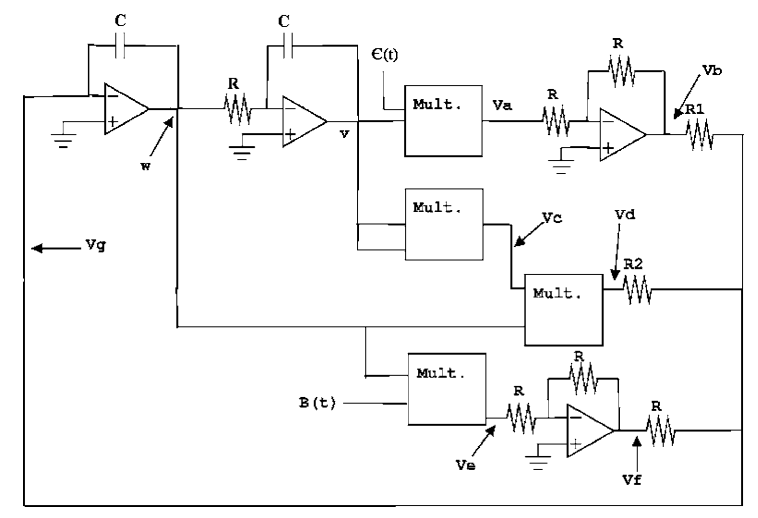
\includegraphics[width=0.7\linewidth]{Images/electronic_syrinx.png}
    \caption{Circuit of the electronic syrinx. This circuit takes into account the the syringial labial position by a dynamical model. Two control parameters are required to drive the system into the oscillation region in the parameters space \cite{electronic_syrinx} }
    \label{fig:electronic_syrinx}
\end{figure}


At this point, the model exhibits great accuracy to generate synthetic birdsongs by just modeling the syrinx as the unique actor in the bird sound production. Keeping the model improvement a new sound production organ actor is added to the model in the same year: the vocal tract (trachea), which is the responsible of the sound filtering \cite{source-source}. Moreover, since the model has new equations and variables it is necessary to study its dynamical behavior to understand what is the dynamical origin of the spectrally birdsongs richness. This articles shown that the spectral content carries a strong signature of the intrinsic dynamics of the sound source, here the sound spectral index (SCI) is introduced to compare the syllables spectral content.\cite{rich}


\begin{minipage}{0.4\linewidth}
\begin{figure}[H]
    \centering
    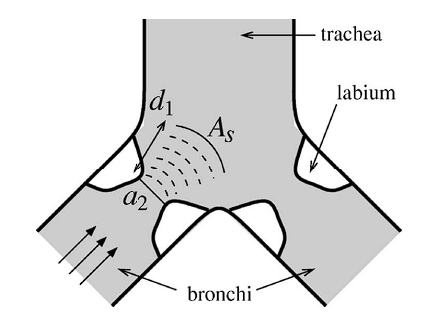
\includegraphics[width=\linewidth]{Images/trachea_coupling.png}
    \caption{Coupling between syrinx labia and vocal tract (trachea). Schematic central cross section. The air sac pressure comes from the bronchis and is modulated by the airflow-induced oscillation of the labia, that then injects a sound pressure wave into the base of the trachea. \cite{source-source}}
    \label{fig:source-source}
\end{figure}    
\end{minipage}\hfill
\begin{minipage}{0.55\linewidth}
\begin{figure}[H]
    \centering
    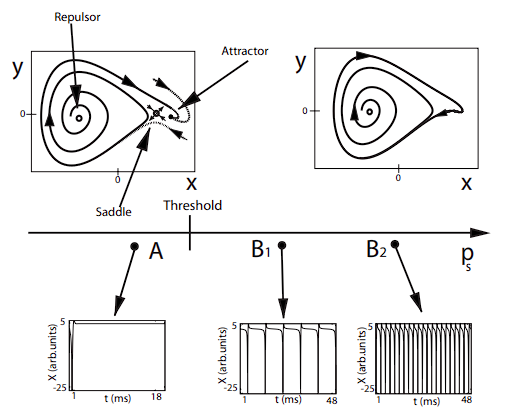
\includegraphics[width=\linewidth]{Images/dynamical_bihavior.png}
    \caption{Bifurcation diagram for the two possible model system dynamics. When the air sac pressure $p_s $ is lower than a threshold the diagram has three fixed points but not labial oscillation occurs, while when the air sac pressure crosses the bifurcation line oscillations born, for values around the threshold the oscillation has zero frequency but for far way values the oscillation starts to be tonal. \cite{rich}}
    \label{fig:dynamical_behavior}
\end{figure}
\end{minipage}
\vspace{10pt}

Complementary to all the research made, in the same year a birdsongs book is published: \textbf{The physics of birdsongs} \cite{book_birdsongs}, that summarize and compile all the information about bird and their sound production models. The book is self-contained, it includes the necessary physical concepts and mathematical background, even it has a chapter about the brain rule in the sound production process. Along with this book, four years later, at 2009, a supporting review of the birdsong models is published in Scholarpedia \cite{scholarpedia_syrinx}.\\


The final actors to be added are the OEC cavity, glottis, and beak. This organs were include until 2011, using a new bifurcation (Bogdanov-Takens), the glottis is modeled as the neck of the Helmholtz resonator representing the OEC that interacts with the atmosphere through the beak. In this articles the physiological instructions from Zebra Finch\footnote{This is song is used since it is widely studied by ornithologist} song are reconstructed, the birdsongs are qualitative compare by computing the SCI and pitch differences, generating highly realistic synthetic songs.\\


Finally, the complete model is published and well describe in the articles \cite{Amador2014\textbf} and \cite{complete_model}. In both articles the dynamical behavior is studied and the Zebra Finch control parameters are computed, they find the space parameters paths that better reproduces the zebra finch songs. \\

Next to the complete model publications, the model has been explored with new ideas to be upgraded as the vortex inclusion in the system dynamics \cite{vortex} or use machine learning tools to analyze and create surrogate birdsongs \cite{ML1, ML2, ML3}.  


\subsection{Current Model}

The previous chapter demonstrated how good is the model, along many years it have been tested and upgraded by the DSL laboratory developing a complete functional vocal bird organ, moreover the syrinx, through a physical model named motor gestures. It consist of simulate the syrinx, trachea, glottis, OEC and beak \cite{complete_model}.

\begin{itemize}
    \item \textbf{Syrinx}
    
    The main character of this model is the syrinx. It is modeled as a mass below the act of an elastic force and a nonlinear damping, defined by the bifurcation theory such that the syrinx movement generate oscillations. Hence, the labia position will satisfy the following second order non-linear differential equation 
    
    \begin{equation*}
        \frac{dx^2}{dt^2} = \gamma^2[-\alpha (t)-\beta (t) x  + x^2 - x^3] - \gamma (1+ x )x\frac{dx}{dy}
    \end{equation*}
    
    making a simple substitution, this equation can be write as set of two first order linear differential equations
    \begin{align}\label{syrinx_edos}
    &\color{mygreen} \frac{dx}{dt} = y\nonumber\\
    &\color{mygreen} \frac{dy}{dt} = \gamma^2[-\alpha (t)-\beta (t) x  + x^2 - x^3] - \gamma (1+ x )xy
    %\\ & \color{mygreen} \frac{dy}{dt} = -\gamma^2\alpha (t)-\gamma^2\beta (t) x + \gamma\big(\gamma[1 - x]x - (1+x)y\big) \nonumber
    % \\ & \color{mygreen} \frac{d^2 x}{dt^2}= f(x(t), x'(t), \alpha(t), \beta(t), \gamma)\quad \text{(Non-linear)} \nonumber
    %\label{oscillator}
\end{align}

The syrinx is modeled with the Bogdanov Takens bifurcation, subsection \ref{Bogdanov_Takens_Bifurcation}, but this is not the only possibility. Another approach is to use a different bifurcation, use another damping function, as was tried in the first model publication \cite{syrinx_first_model}.\\ 

To study the ODEs bifurcations let us start to calculating the equilibrium points. This points occurs when the variables derivatives are zero
\begin{gather*}
    \frac{dx}{dt} = y = 0\\
    \frac{dy}{dt} = \gamma^2[-\alpha (t)-\beta (t) x  + x^2 - x^3] - \gamma (1+ x )xy = 0\\
    \Rightarrow \quad \gamma^2[-\alpha (t)-\beta (t) x  + x^2 - x^3] = 0 
\end{gather*}

Then, the derivatives vanishes when the labial velocity is zero (curve $y=0$) and the air sac pressure and labial tension satisfies the previous relation that can be solved for $\alpha$
\begin{equation}\label{alpha_solve}
    \alpha (t) = -\beta (t) x  + x^2 - x^3 
\end{equation}
Thinking geometrically, this is equivalent to find if and where the two curves intersect: the horizontal line define by the air sac pressure $g(x)=\alpha$ and the labial position condition  define by the cubic polynomial $f(x)=-\beta x  + x^2 - x^3 $. In order to get oscillations the tangent of the functions must be equal and the control parameters must satisfies the relation $0=-\beta+2x-3x^2$ which give a solution for the parameter $\beta$ that later are used for calculate the bifurcations curves present in the Takens Bogdanov, two saddle-node and one hotf  bifurcations curves.



\item \textbf{Trachea (windpipe)}

The trachea acts as a filter and is modeled as a tube with one end opened \cite{trachea_birdsong}, the end connected to the syrinx, and the other one closed, the end that is connected to the glottis. The output pressure of the trachea satisfies a delayed differential equation of the input pressure, they are proportional directly. Furthermore, since the wave can be absorbed and reflected by the trachea a reflection coefficient is defined $r$ such that output pressure is 
\begin{gather}\label{trache_edos}
\color{myyellow} p_i (t) = A y(t) + p_{back}\left( t - \frac{L}{c} \right)\quad ; \quad p_{back} (t) = -r p_i\left( t - \frac{L}{c} \right)\\
\color{myyellow} p_{out} (t) = (1-r)p_i\left( t - \frac{L}{c} \right)\\
\color{myyellow} \frac{d p_{out}}{dt} (t) = \frac{p_{out}(t)- p_{out}(t-dt)}{dt}
%\\ \color{myyellow}\frac{dp_{out}}{dt} = g(x'(t), p_{in}(t), p_{in}(t-dt))
\end{gather}

here $p_{back}$ is the backward pressure, $L$ the trachea length, and $c$ the velocity of the sound in air. The last equation is the the approximation by backward difference of the output pressure derivative.
    
    \item  \textbf{Beak, Glottis, and Oro-Oesophageal Cavity  (OEC)}
    
    Previous works showed how a simple circuit can simulate the filtering audio process done by the birds \cite{OEC_units, OEC_circuit} : the glottis is modeled with a resistor; the OEC as a Helmholtz resonator with an inductance and a resistor; and the beak as an inductance in series with a resistor. Since the the filtering circuit, Figure \ref{fig:mallas}, is analog to the filtering bird process, the current is equivalent to the pressure and hence there will be an analog Kirchhoff voltage law for the pressure

    \begin{figure}[H]
    \centering
    \begin{minipage}{.48\linewidth}
        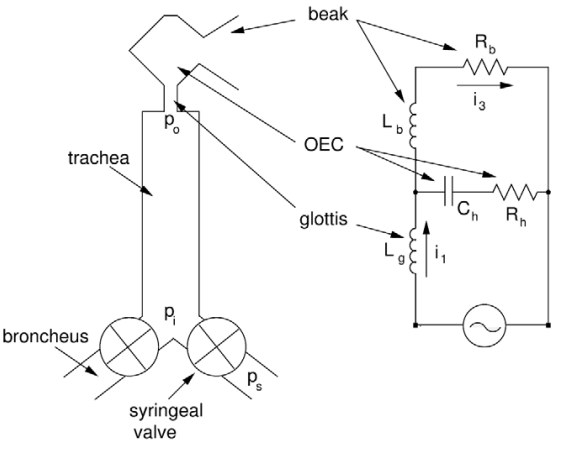
\includegraphics[width=\linewidth]{Images/OEC.png}
        \caption{\cite{OEC_currents}}
        \label{fig:oec_old}
    \end{minipage}
    \hfill
    \begin{minipage}{.48\linewidth}
        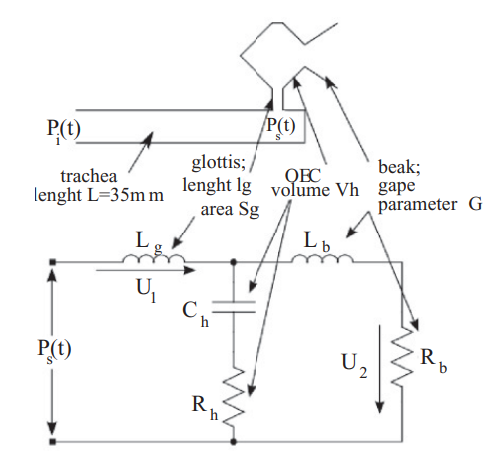
\includegraphics[width=\linewidth]{Images/oec_new.png}
        \caption{\cite{OEC_circuit}}
        \label{fig:oec_new}
    \end{minipage}
    \end{figure}    
    
    \vspace{5pt}
    
    \begin{minipage}{0.25\textwidth}
        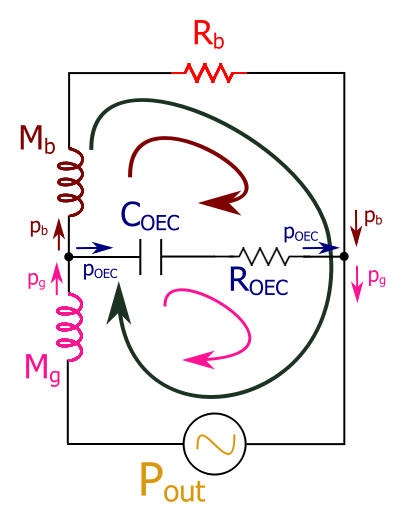
\includegraphics[scale=1.2]{Images/mallas.png}
    \captionof{figure}{Analog voltage Kirchhoff loops.}\label{fig:mallas}
    \end{minipage} \hspace{1pt}
    \begin{minipage}{0.6\textwidth}
    using an analog acoustical Kirchhoff voltage law in all the loops\\
        \begin{gather}
        \color{mypink} p_{out} = M_g p_g'+ \frac{1}{C_{OEC}} \int p_{OEC} dt +R_{OEC} \; p_{OEC}\\ %\color{pink}
        \color{myred}M_b p_b'+R_bp_b+\frac{1}{C_{OEC}}\int p_{OEC} dt +R_{OEC} \; p_{OEC}=0\\
        \color{mygreen}p_{out} = M_g p_g'+M_bp_b'+R_bp_b\\
        p_g = p_b+p_{OEC}
    \end{gather}
    \vspace{50pt}
    \end{minipage}
    
    taking the derivative respect to time
    \begin{equation}\label{OEC_loops_derivatives}
        \begin{gathered}
            \color{mypink} M_g p_g''+ \frac{1}{C_{OEC}}\; p_{OEC} +R_{OEC} \; p_{OEC}'- p_{out}'  = 0\\ %\color{pink}
        \color{myred} M_b p_b''+R_b p_b'+\frac{1}{C_{OEC}} \; p_{OEC} + R_{OEC} \; p_{OEC}'=0\\
        \color{mygreen}p_{out}' = M_g p_g''+M_bp_b''+R_bp_b'
        \end{gathered}
    \end{equation}
    
    
    % \begin{equation}
    % \vcenter{\hbox{\begin{minipage}{0.3\textwidth}
    % \centering
    % 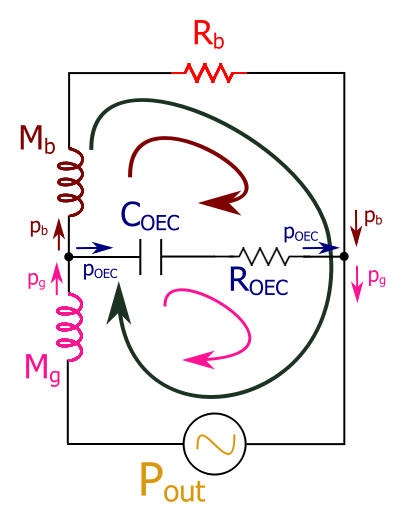
\includegraphics[scale=1.5]{Images/mallas.png}
    % \captionof{figure}{Loops used with the Kirchhoff voltage equivalent law.}
    % \end{minipage}}}
    % \qquad\qquad
    % \begin{gathered}\label{OEC_loops_derivatives}
    % \color{mypink} M_g p_g''+ \frac{1}{C_{OEC}}\; p_{OEC} +R_{OEC} \; p_{OEC}'- p_{out}'  = 0\\ %\color{pink}
    %     \color{myred} M_b p_b''+R_b p_b'+\frac{1}{C_{OEC}} \; p_{OEC} + R_{OEC} \; p_{OEC}'=0\\
    %     \color{mygreen}p_{out}' = M_g p_g''+M_bp_b''+R_bp_b'
    % \end{gathered}
    % \end{equation}
    
    making a change of variable and solving the last equation for $p_b'$ 
    \begin{gather}\label{derivate_b_dpg}
        p_{g}' = dp_{g} , \qquad p_{g}'' =  dp_{g}' \\ \label{derivate_b}
        \color{mygreen} 
        p_b'= \frac{1}{M_b}\left[ p_{out}-R_bp_b-M_{g}p_{g}'\right] = \frac{1}{M_b}\left[ p_{out}-R_bp_b-M_{g}dp_{g}\right]
        %\\ \color{mygreen} p_b''= \frac{1}{M_b}\left[ p_{out}'-R_bp_b'-M_{g}dp_{g}'\right]
    \end{gather}
    changing the pink equation to 
    \begin{gather*}
         M_g p_g''+ \frac{1}{C_{OEC}}\; (p_g-p_b) +R_{OEC} \; (p_g'-p_b')- p_{out}'  = 0\\
         M_g dp_g'= -\frac{1}{C_{OEC}}\; p_g+\frac{1}{C_{OEC}}\;p_b -R_{OEC} \; dp_g+ R_{OEC} \frac{1}{M_b}\left[ p_{out}-R_bp_b-M_{g}dp_{g}\right] + p_{out}'\\
         M_g dp_g'= -\frac{1}{C_{OEC}}\; p_g+\left(\frac{1}{C_{OEC}} -\frac{R_{OEC}R_b}{M_b}\right)p_b -R_{OEC}\left(1+\frac{M_g}{M_b}\right) dp_g+  \frac{R_{OEC}}{M_b} p_{out} + p_{out}'
    \end{gather*}
    
    solving for $dp_g'$
    \begin{multline}\label{derivative_glotis}
         dp_g'= -\frac{1}{C_{OEC}M_g}\; p_g+\frac{1}{M_g}\left(\frac{1}{C_{OEC}} -\frac{R_{OEC}R_b}{M_b}\right)p_b \\
         -R_{OEC}\left(\frac{1}{M_g}+
         \frac{1}{M_b}\right) dp_g +  \frac{R_{OEC}}{M_bM_g} p_{out} + \frac{1}{M_g}p_{out}'
    \end{multline}
    
    Hence, the set of first order differential equations that simulate the whole filtering bird organ are defined by the equations\eqref{derivate_b_dpg}, \eqref{derivate_b} and \eqref{derivative_glotis}
    \begin{align}\label{OEC_edos}
        \frac{d}{dt} p_g &= p_g'= dp_g \nonumber\\
        \frac{d}{dt} dp_g  &= dp_g'= -\frac{1}{C_{OEC} M_g}p_g  - R_{OEC} \left( \frac{1}{M_b} + \frac{1}{M_g}\right) dp_g + \frac{1}{M_g}\left( \frac{1}{C_{OEC} } + \frac{R_{OEC} R_b}{ M_b}\right) p_b \nonumber\\
        &  \qquad \qquad + \frac{1}{M_g}\frac{dp_{out} }{dt} + \frac{R_{OEC}}{M_g M_b  }  p_{out} \nonumber\\
        \frac{d}{dt} p_b &= p_b' = -  \frac{M_g}{M_b}  p_g' - \frac{R_b}{M_b} p_b + \frac{1}{M_b} p_{out}
        %\\  & \color{myblue} \frac{d\vec{p}}{dt} = \vec{h}(\vec{p},  p_{out}, p_{out}'), \quad \vec{p} = (p_g, p_g', p_b)
    \end{align}
    
    with $M$, $R$, and $C$ denoting the Intertance, Resistance, and Compilance, acoustical analogs of Impedance $L$, Resistance, and Capacitance, electrical variables, respectively. The length and area of an element $a$ are $l_a$ and $S_a$, respectively, which in our model stand for the beak (b), the glottis (g), and the OEC volume (OEC) \cite{OEC_currents, OEC_circuit}.
    
\begin{figure}[H]
    \centering
    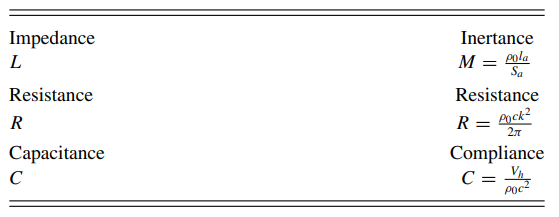
\includegraphics[scale=0.55]{Images/acoustic_analog.png}
    \caption{Acoustic and electrical analogs \cite{OEC_circuit} }
    \label{fig:bird_sound_organs}
\end{figure}
    
    
    reference \cite{Neuromuscular}, \cite{birdsongs_ML_new}, \cite{muscles_role}, 

\end{itemize}



\subsection{State of Art}

Currently, the model is being used to train machine learning (ML) algorithms to identify and generate bird songs, and even its dynamical behavior is still being studied with ML ideas.\\

The model automatizing has been discussed from many years ago. The first article that proposed a solution method to find the parameters automatically was published in 2015, \cite{automatization}, where the idea is to produces a grid for the control parameters and calculate at each node of the grid the Spectral Content Index (SCI) and the Fundamental Frequency (FF or pitch) to find what are the control parameters values, the motor gesture (synthetic audio), that generates a good approximation of the real birdsong, this grid computation is done previously and is stored in data files. \\

New article research shows how neural networks can help to solve the problem of automatizing parameters using as input data the neural population activity recorded from electrode arrays implanted in the
premotor nucleus HVC \cite{NNbirds}. \\

The present work presents, describes and evaluate a computational physical model to automatize the motor gestures generation from audio data recorded. In addition, the model is implemented as python package, using POO thinking to the implementation and Github to storage, such that make it easily to use, to share and develop.

%for biologist, ornithologist, and computer escientest  



%\subsection{Preset Works}
% \subsection{Future Applications}

% Some of the future works for this work are:

% \begin{itemize}
%     \item Classify and identify birds by their motor gestures curves.
%     \item Generate a synthetic songbirds collection with audio signals and optimal parameters.
%     \item Improve the optimization objective function implementation and theory definition. If the model could be expressed as a single differential operator, a  better optimization algorithms can be used to solve the problem but they require first and second derivatives, the Jacobian and Hessian.
% \end{itemize} 


\section{Automatizing}

The final step for the model is make it automatic an portable: that any person can download an efficient implementation of the model as package, easy to use and fast to execute. This objective can be achieve by designing, implementing an evaluating a computational physical model that given an audio signal it 

\begin{itemize}
    \item Characterize the audio signal by computing its fundamental frequency (FF), also called pitch, and its tempo-spectral features.
    \item Generate a synthetic syllable from the input signal and some model parameters ($\alpha, \beta, \gamma$).
    \item Compare the real and synthetic signals.
    \item Find the best optimal parameters values that better simulate the real syllable (birdsong).
    \item Split an audio song into single syllables.
    \item Write an audio file with the synthetic syllable (song).
\end{itemize}

The final result is an available online package that generates synthetic birdsongs from real audio data, by using recorded birdsongs in audio wav format. This package allows not just to generate the most similar synthetic birdsong, it also offers the possibility to generate a huge amount of syllables related to the real audio. Moreover, the model implementation allows to change the bifurcation, using symbolic calculus, and explore the physical model behavior, by varying the system variables values ($\alpha, \beta, \gamma$).

\subsection{Optimization Problem}

The goal of this work is to find automatically some optimal parameters from experimental samples, real audios. This can be formulated as an inverse problem with a white box\footnote{physical model where the behavior is well known, motor gestures}, the goal is to find the optimal parameters that causes the measured observations using the white box model. Since the problem is not linear the optimal parameters may not be unique. \\

This kind of problems have been studied from many years ago and there are many theories created to solve them, one of these theories is the numerical optimization that offers a new tool to solve a wide variety of inverse problems by defining them as a minimization (or maximization) optimization problem.\\

Using the numerical optimization theory, the motors gestures automatizing problem can be formulated as the following minimization that dependes of three control parameters: air-sac pressure $\alpha$, labial tension $\beta$, and a constant time $\gamma$, two vector arrays and one real number respectively.

%This change of paradigm gives a big advantage in fact since the 
\begin{equation}\label{opt_general}
\begin{aligned}
\underset{ \gamma \in \mathbb{R},\; \alpha,\beta\in \mathbb{R}^n}{\text{min}} &\qquad  ||\hat{SCI}_{real} - \hat{SCI}_{synt} ( \gamma,\alpha,\beta)||_2  + || (\hat{FF}_{real} - \hat{FF}_{synt}(\gamma,\alpha,\beta)||_2 \\
    & \qquad \qquad  - corr(FC_{real},FC_{synt}(\gamma, \alpha, \beta)) \\
    \text { subject to }  & \qquad \gamma \in \Omega_\gamma, \quad  \beta \in \Omega_\beta ,  \quad  \alpha \in \Omega_\alpha
\end{aligned}
\end{equation}

Here $corr$ is the acoustic dissimilarity between two spectral coefficients sets, $FC$ the Fourier spectral coefficients, $\hat{FF}$ the dimensionless fundamental frequency (divide by $1 \; kHz$ and its size), $\hat{SCI}$ the spectral content index divide by its size, and $\Omega_i$ represents the feasible region for the variable $i$.\\

This minimization problem is nonlinear, then nonlinear optimization algorithms are required, and unconstrained. However, the Jacobian and Hessian matrix calculations are not simple and require a deeper study in order to be able to implement better algorithms and be ensure of the convergence to a solution. Further techniques can also involve constraints, in this problem the most appropriated constraints are the bifurcations curves of the labia position.